% Created by tikzDevice version 0.12.6 on 2026-03-18 00:13:13
% !TEX encoding = UTF-8 Unicode
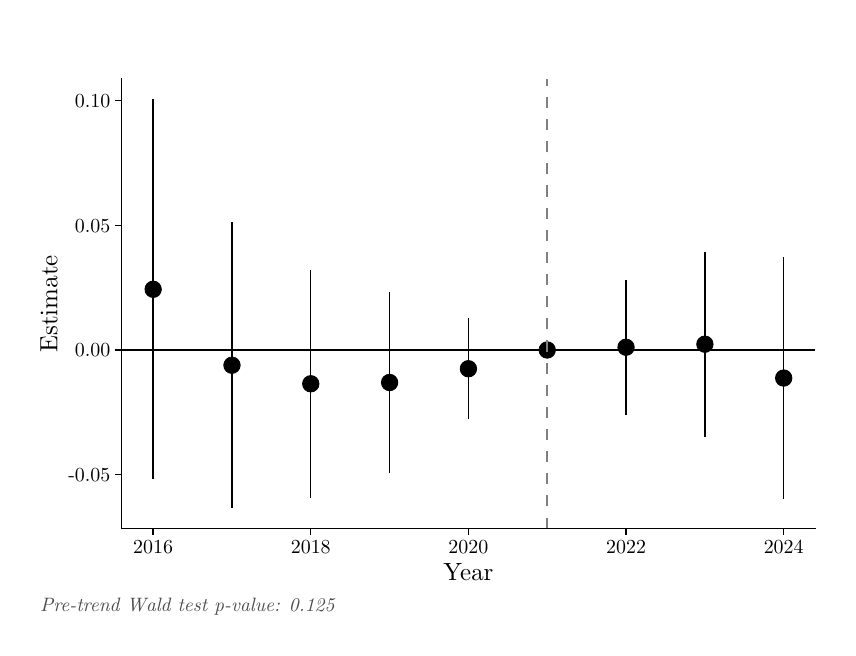
\begin{tikzpicture}[x=1pt,y=1pt]
\definecolor{fillColor}{RGB}{255,255,255}
\path[use as bounding box,fill=fillColor,fill opacity=0.00] (0,0) rectangle (289.08,216.81);
\begin{scope}
\path[clip] (  0.00,  0.00) rectangle (289.08,216.81);
\definecolor{drawColor}{RGB}{255,255,255}
\definecolor{fillColor}{RGB}{255,255,255}

\path[draw=drawColor,line width= 0.5pt,line join=round,line cap=round,fill=fillColor] (  0.00,  0.00) rectangle (289.08,216.81);
\end{scope}
\begin{scope}
\path[clip] ( 33.94, 35.79) rectangle (284.58,198.27);
\definecolor{fillColor}{RGB}{255,255,255}

\path[fill=fillColor] ( 33.94, 35.79) rectangle (284.58,198.27);
\definecolor{drawColor}{RGB}{0,0,0}

\path[draw=drawColor,line width= 0.3pt,dash pattern=on 4pt off 4pt ,line join=round] (187.74, 35.79) -- (187.74,198.27);

\path[draw=drawColor,line width= 0.3pt,line join=round] ( 33.94,100.34) -- (284.58,100.34);

\path[draw=drawColor,line width= 0.5pt,line join=round] ( 45.34, 53.66) -- ( 45.34,190.89);

\path[draw=drawColor,line width= 0.5pt,line join=round] ( 73.82, 43.17) -- ( 73.82,146.48);

\path[draw=drawColor,line width= 0.5pt,line join=round] (102.30, 46.85) -- (102.30,129.41);

\path[draw=drawColor,line width= 0.5pt,line join=round] (130.78, 56.00) -- (130.78,121.18);

\path[draw=drawColor,line width= 0.5pt,line join=round] (159.26, 75.33) -- (159.26,111.80);

\path[draw=drawColor,line width= 0.5pt,line join=round] (187.74,100.34) -- (187.74,100.34);

\path[draw=drawColor,line width= 0.5pt,line join=round] (216.22, 77.01) -- (216.22,125.65);

\path[draw=drawColor,line width= 0.5pt,line join=round] (244.71, 68.97) -- (244.71,135.88);

\path[draw=drawColor,line width= 0.5pt,line join=round] (273.19, 46.55) -- (273.19,133.86);
\definecolor{fillColor}{RGB}{0,0,0}

\path[draw=drawColor,line width= 0.3pt,line join=round,line cap=round,fill=fillColor] ( 45.34,122.27) circle (  2.97);

\path[draw=drawColor,line width= 0.3pt,line join=round,line cap=round,fill=fillColor] ( 73.82, 94.83) circle (  2.97);

\path[draw=drawColor,line width= 0.3pt,line join=round,line cap=round,fill=fillColor] (102.30, 88.13) circle (  2.97);

\path[draw=drawColor,line width= 0.3pt,line join=round,line cap=round,fill=fillColor] (130.78, 88.59) circle (  2.97);

\path[draw=drawColor,line width= 0.3pt,line join=round,line cap=round,fill=fillColor] (159.26, 93.56) circle (  2.97);

\path[draw=drawColor,line width= 0.3pt,line join=round,line cap=round,fill=fillColor] (187.74,100.34) circle (  2.97);

\path[draw=drawColor,line width= 0.3pt,line join=round,line cap=round,fill=fillColor] (216.22,101.33) circle (  2.97);

\path[draw=drawColor,line width= 0.3pt,line join=round,line cap=round,fill=fillColor] (244.71,102.43) circle (  2.97);

\path[draw=drawColor,line width= 0.3pt,line join=round,line cap=round,fill=fillColor] (273.19, 90.20) circle (  2.97);

\path[draw=drawColor,line width= 0.6pt,line join=round] ( 33.94,100.34) -- (284.58,100.34);
\definecolor{drawColor}{gray}{0.50}

\path[draw=drawColor,line width= 0.6pt,dash pattern=on 4pt off 4pt ,line join=round] (187.74, 35.79) -- (187.74,198.27);
\end{scope}
\begin{scope}
\path[clip] (  0.00,  0.00) rectangle (289.08,216.81);
\definecolor{drawColor}{RGB}{0,0,0}

\path[draw=drawColor,line width= 0.5pt,line join=round,line cap=rect] ( 33.94, 35.79) --
	( 33.94,198.27);
\end{scope}
\begin{scope}
\path[clip] (  0.00,  0.00) rectangle (289.08,216.81);
\definecolor{drawColor}{RGB}{0,0,0}

\node[text=drawColor,anchor=base east,inner sep=0pt, outer sep=0pt, scale=  0.72] at ( 29.89, 52.78) {-0.05};

\node[text=drawColor,anchor=base east,inner sep=0pt, outer sep=0pt, scale=  0.72] at ( 29.89, 97.87) {0.00};

\node[text=drawColor,anchor=base east,inner sep=0pt, outer sep=0pt, scale=  0.72] at ( 29.89,142.95) {0.05};

\node[text=drawColor,anchor=base east,inner sep=0pt, outer sep=0pt, scale=  0.72] at ( 29.89,188.04) {0.10};
\end{scope}
\begin{scope}
\path[clip] (  0.00,  0.00) rectangle (289.08,216.81);
\definecolor{drawColor}{RGB}{0,0,0}

\path[draw=drawColor,line width= 0.5pt,line join=round] ( 31.69, 55.26) --
	( 33.94, 55.26);

\path[draw=drawColor,line width= 0.5pt,line join=round] ( 31.69,100.34) --
	( 33.94,100.34);

\path[draw=drawColor,line width= 0.5pt,line join=round] ( 31.69,145.43) --
	( 33.94,145.43);

\path[draw=drawColor,line width= 0.5pt,line join=round] ( 31.69,190.52) --
	( 33.94,190.52);
\end{scope}
\begin{scope}
\path[clip] (  0.00,  0.00) rectangle (289.08,216.81);
\definecolor{drawColor}{RGB}{0,0,0}

\path[draw=drawColor,line width= 0.5pt,line join=round,line cap=rect] ( 33.94, 35.79) --
	(284.58, 35.79);
\end{scope}
\begin{scope}
\path[clip] (  0.00,  0.00) rectangle (289.08,216.81);
\definecolor{drawColor}{RGB}{0,0,0}

\path[draw=drawColor,line width= 0.5pt,line join=round] ( 45.34, 33.54) --
	( 45.34, 35.79);

\path[draw=drawColor,line width= 0.5pt,line join=round] (102.30, 33.54) --
	(102.30, 35.79);

\path[draw=drawColor,line width= 0.5pt,line join=round] (159.26, 33.54) --
	(159.26, 35.79);

\path[draw=drawColor,line width= 0.5pt,line join=round] (216.22, 33.54) --
	(216.22, 35.79);

\path[draw=drawColor,line width= 0.5pt,line join=round] (273.19, 33.54) --
	(273.19, 35.79);
\end{scope}
\begin{scope}
\path[clip] (  0.00,  0.00) rectangle (289.08,216.81);
\definecolor{drawColor}{RGB}{0,0,0}

\node[text=drawColor,anchor=base,inner sep=0pt, outer sep=0pt, scale=  0.72] at ( 45.34, 26.78) {2016};

\node[text=drawColor,anchor=base,inner sep=0pt, outer sep=0pt, scale=  0.72] at (102.30, 26.78) {2018};

\node[text=drawColor,anchor=base,inner sep=0pt, outer sep=0pt, scale=  0.72] at (159.26, 26.78) {2020};

\node[text=drawColor,anchor=base,inner sep=0pt, outer sep=0pt, scale=  0.72] at (216.22, 26.78) {2022};

\node[text=drawColor,anchor=base,inner sep=0pt, outer sep=0pt, scale=  0.72] at (273.19, 26.78) {2024};
\end{scope}
\begin{scope}
\path[clip] (  0.00,  0.00) rectangle (289.08,216.81);
\definecolor{drawColor}{RGB}{0,0,0}

\node[text=drawColor,anchor=base,inner sep=0pt, outer sep=0pt, scale=  0.90] at (159.26, 16.93) {Year};
\end{scope}
\begin{scope}
\path[clip] (  0.00,  0.00) rectangle (289.08,216.81);
\definecolor{drawColor}{RGB}{0,0,0}

\node[text=drawColor,rotate= 90.00,anchor=base,inner sep=0pt, outer sep=0pt, scale=  0.90] at ( 10.70,117.03) {Estimate};
\end{scope}
\begin{scope}
\path[clip] (  0.00,  0.00) rectangle (289.08,216.81);
\definecolor{drawColor}{gray}{0.30}

\node[text=drawColor,anchor=base west,inner sep=0pt, outer sep=0pt, scale=  0.70] at (  4.50,  5.86) {\itshape Pre-trend Wald test p-value: 0.125};
\end{scope}
\end{tikzpicture}
